% !TeX program = pdflatex
% !TeX encoding = utf8
% !TeX spellcheck = uk_UA
% !BIB program = bibtex8

\documentclass[18pt]{LectMechanics}
\title[Physics 1]{\huge\bfseries Units, Physical Quantities, and Vectors}
\date{}
\begin{document}
%=======================================================================================================
%\usebackgroundtemplate{
%
%\tikz\node[opacity=0.3]{\includegraphics[width=\paperwidth,height=\paperheight]{background}};%
%}
\begin{frame}
	\titlepage
\end{frame}
%=======================================================================================================
\usebackgroundtemplate{
}





%=======================================================================================================
\begin{frame}{Goals for Lecture}{}
	\begin{itemize}
		\item To learn three fundamental quantities of physics and the units to
		      measure them
		\item To keep track of significant figures in calculations
		\item To understand vectors and scalars and how to add vectors graphically
		\item To determine vector components and how to use them in calculations
		\item To understand unit vectors and how to use them with components to
		      describe vectors
		\item To learn two ways of multiplying vectors
	\end{itemize}
\end{frame}
%=======================================================================================================




%=======================================================================================================
\begin{frame}{What is Physics}{}
	\begin{boxedframe}{Political Factors}
		Physics is an experimental science in which physicists seek patterns that
		relate the phenomena of nature.
	\end{boxedframe}
	\begin{itemize}
		\item The patterns are called \emph{physical theories}.
		\item A very well established or widely used theory is called a
		      \emphbox{physical law} or \emphbox{principle}.
	\end{itemize}
\end{frame}

%=======================================================================================================




%=======================================================================================================
\begin{frame}{Standards and units}{}
	\begin{itemize}
		\item \emph{Length}, \emph{time}, and \emph{mass} are three fundamental
		      quantities of physics.
		\item The International System (SI for Système International) is the most
		      widely used system of units.
		\item In SI units, length is measured in \textit{meters}, time in
		      \textit{seconds}, and mass in \textit{kilograms}.
	\end{itemize}
\end{frame}
%=======================================================================================================



%=======================================================================================================
\begin{frame}{Unit prefixes}{}
	\begin{center}
		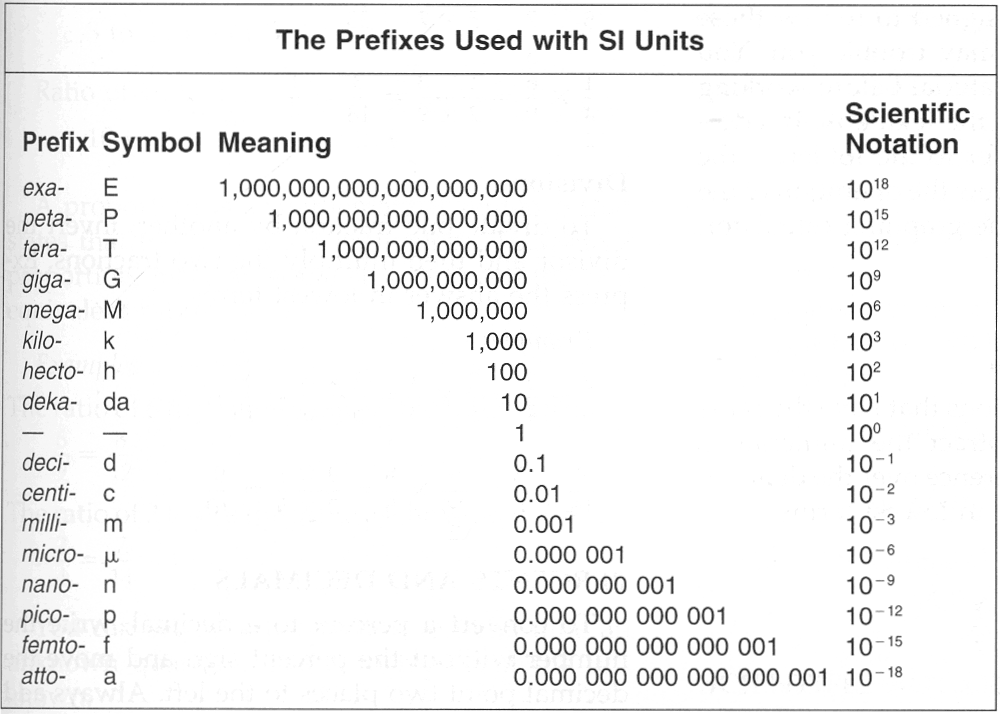
\includegraphics[width=0.8\linewidth]{Unit_prefixes}
	\end{center}

\end{frame}
%=======================================================================================================


%=======================================================================================================
\begin{frame}{Vectors and scalars}{}
	\begin{itemize}
		\item A \emph{scalar quantity} can be described by a \textit{single number}.
		\item A \emph{vector quantity} has both a \textit{magnitude} and a
		      \textit{direction in space}.
		\item A vector quantity is represented in italic type with an arrow over it:
		      $\vec A$.
		\item The magnitude of $\vec A$ is written as $A$ or $|\vec A|$.
	\end{itemize}
\end{frame}
%=======================================================================================================

%=======================================================================================================
\begin{frame}{Adding two vectors}{}
	\begin{center}
		Two vectors may be added graphically using either the \emph{parallelogram
			method} or the \emph{head-to-tail method}.
	\end{center}
	\begin{center}
		\begin{minipage}{.3\textwidth}
			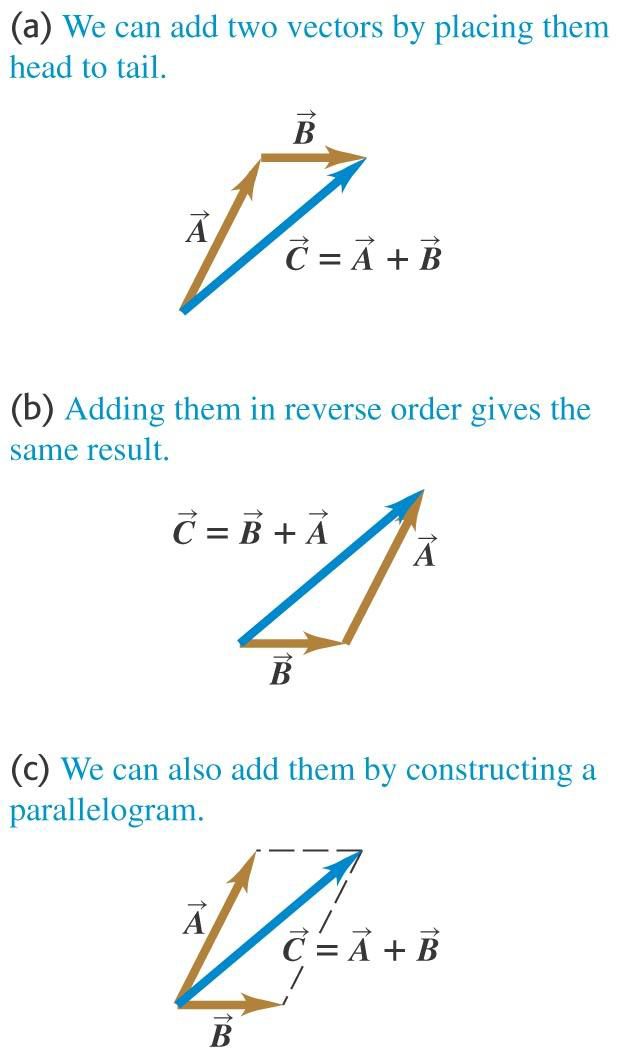
\includegraphics[width=\linewidth]{Vector_Addition_1}
		\end{minipage}\
		\begin{minipage}{.3\textwidth}
			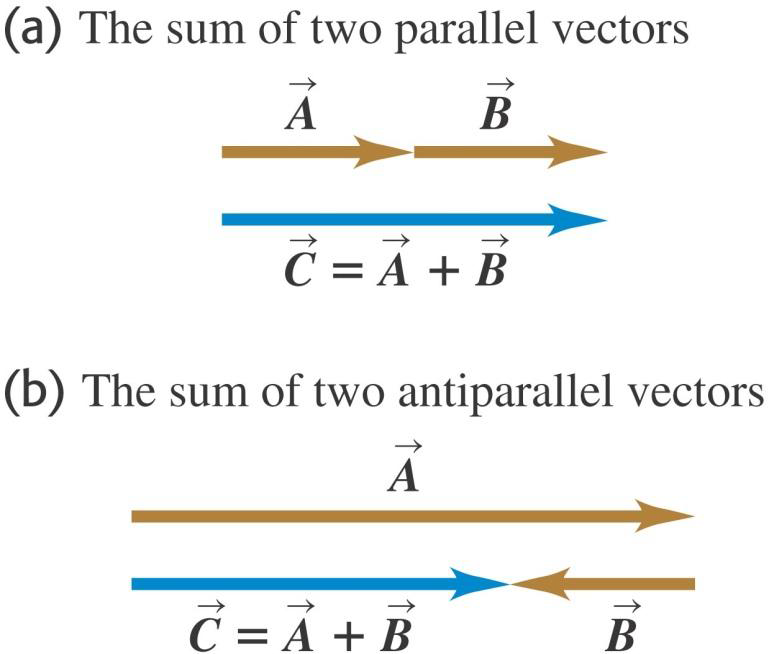
\includegraphics[width=\linewidth]{Vector_Addition_2}
		\end{minipage}
	\end{center}
\end{frame}

%=======================================================================================================

%=======================================================================================================
\begin{frame}[t]{Adding more than two vectors graphically}{}
	To add several vectors, use the head-to-tail method.
	\begin{center}
		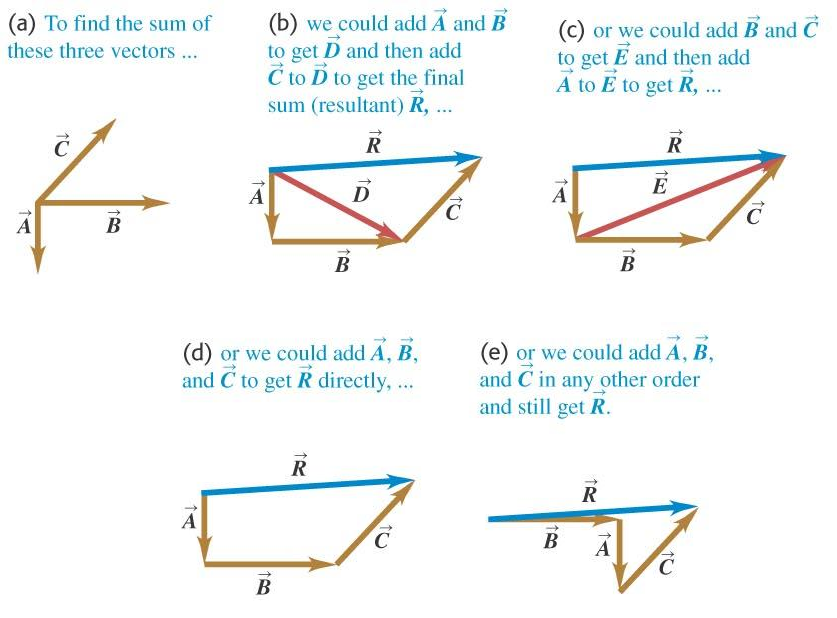
\includegraphics[width=0.7\linewidth]{Vector_Addition_3}
	\end{center}
\end{frame}
%=======================================================================================================

%=======================================================================================================
\begin{frame}{Subtracting vectors}{}
	\begin{center}
		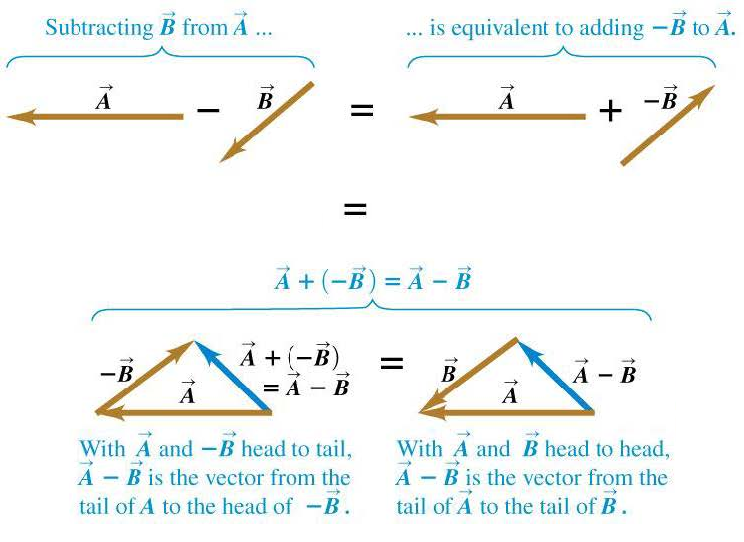
\includegraphics[width=0.8\linewidth]{Substracting_vectors}
	\end{center}
\end{frame}
%=======================================================================================================


%=======================================================================================================
\begin{frame}{Multiplying a vector by a scalar}{}
	If $c$ is a scalar, the product $c\vec A$ has magnitude $cA$.


	\begin{center}
		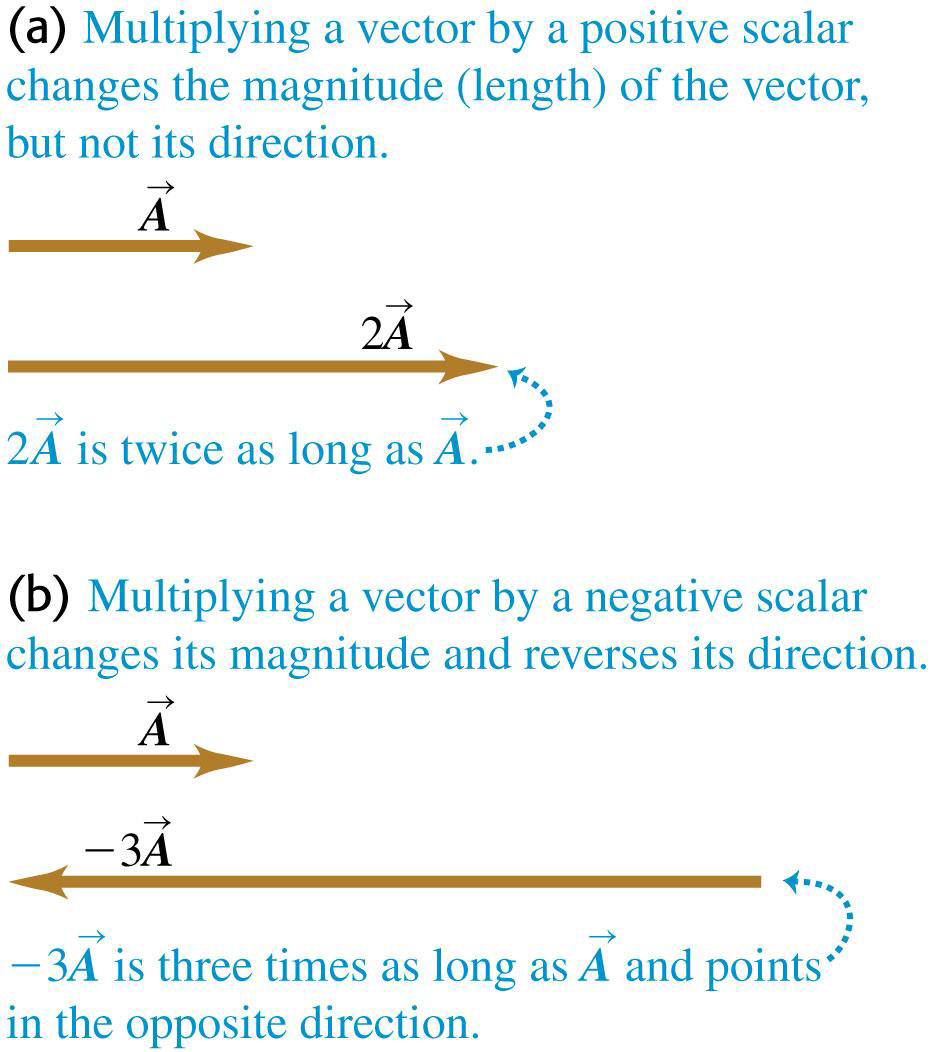
\includegraphics[width=0.4\linewidth]{Multiplying_by_scalar}
	\end{center}
\end{frame}
%=======================================================================================================



%=======================================================================================================
\begin{frame}{Components of a vector}{}
	\begin{enumerate}
		\item Adding vectors graphically provides limited accuracy. Vector components
		      provide a general method for adding vectors.
		\item Any vector can be represented by an $x$-component $A_x$ and a
		      $y$-component $A_y$.
		\item Use trigonometry to find the components of a vector: $A_x = A\cos\theta$
		      and $A_y = A\sin\theta$, where $\theta$ is measured from the $+x$-axis toward
		      the $+y$-axis.
	\end{enumerate}
	\begin{center}
		\includegraphics[width=\linewidth]{Vector_components}
	\end{center}
\end{frame}
%=======================================================================================================



%=======================================================================================================
\begin{frame}{Magnitude and components of the vector}{}
	We can use the components of a vector to find its magnitude and direction:
	\begin{equation*}
		\tcbhighmath[drop fuzzy shadow]{A = \sqrt{A_x^2 + A_y^2}}, \tcbhighmath[drop fuzzy shadow]{\tan\theta = \frac{A_x}{A_y}}
	\end{equation*}
	\begin{center}
		\includegraphics[width=\linewidth]{Vector_components}
	\end{center}
\end{frame}
%=======================================================================================================

%=======================================================================================================
\begin{frame}{Unit vectors}{}
	\begin{columns}
		\begin{column}{.4\linewidth}
			\begin{enumerate}
				\item  A unit vector has a magnitude
				      of $1$ with no units.
				\item The unit vector $\vec i$ points in the
				      $+x$-direction,

				      $\vec j$ points in the $+y$ - direction,

				      $\vec k$ points in the $+z$-direction.
				\item Any vector can be expressed in terms of its components as
				      \begin{equation*}
					      \tcbhighmath[drop fuzzy shadow]{\vec A = A_x\vec i + A_y\vec j + A_x \vec k}
				      \end{equation*}
			\end{enumerate}
		\end{column}
		\begin{column}{.4\linewidth}
			\begin{center}
				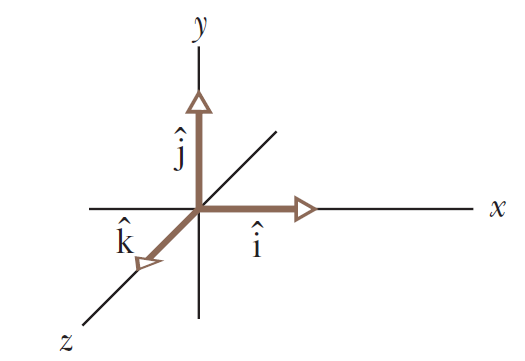
\includegraphics[width=\linewidth]{unit_vectors}
			\end{center}
		\end{column}
	\end{columns}
\end{frame}
%=======================================================================================================

%=======================================================================================================
\begin{frame}[t]{The scalar product}{}
	\begin{columns}
		\begin{column}{0.5\linewidth}
			The scalar (or dot) product of two vectors $\vec a$ and $\vec b$ is written as $\vec a \cdot \vec b$ and is the scalar quantity given by:
			\begin{equation*}
				\tcbhighmath[drop fuzzy shadow]{\vec a \cdot \vec b = ab\cos\phi}
			\end{equation*}
		\end{column}
		\begin{column}{0.5\linewidth}
			\begin{center}
				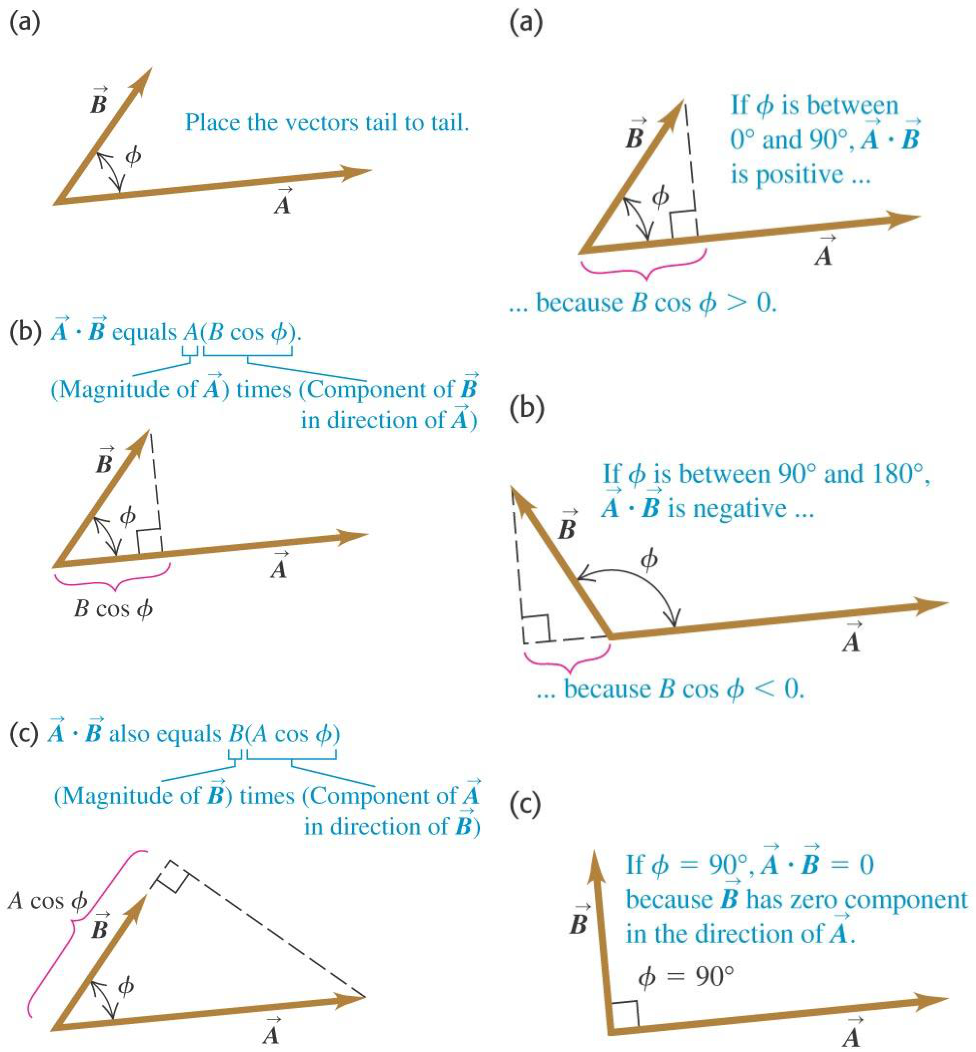
\includegraphics[width=\linewidth]{Scalar_prod}
			\end{center}
		\end{column}
	\end{columns}

\end{frame}
%=======================================================================================================

%=======================================================================================================
\begin{frame}{The scalar product via components}{}
	In terms of components the scalar product can be calculated as:
	\begin{equation*}
		\tcbhighmath[drop fuzzy shadow]{\vec a \cdot \vec b = a_x b_x + a_yb_y + a_zb_z}
	\end{equation*}
\end{frame}
%=======================================================================================================

%=======================================================================================================
\begin{frame}[t]{The vector product}{}
\begin{columns}
	\begin{column}{0.4\linewidth}
		The vector (or cross) product of two vectors $\vec a$ and $\vec b$ is written as $\vec a \times \vec b$ and is the vector whose magnitude is given by:
		\begin{equation*}
		\tcbhighmath[drop fuzzy shadow]{|\vec a \times \vec b| = ab\sin\phi}
		\end{equation*}
	\end{column}
	\begin{column}{0.6\linewidth}
		\begin{center}
			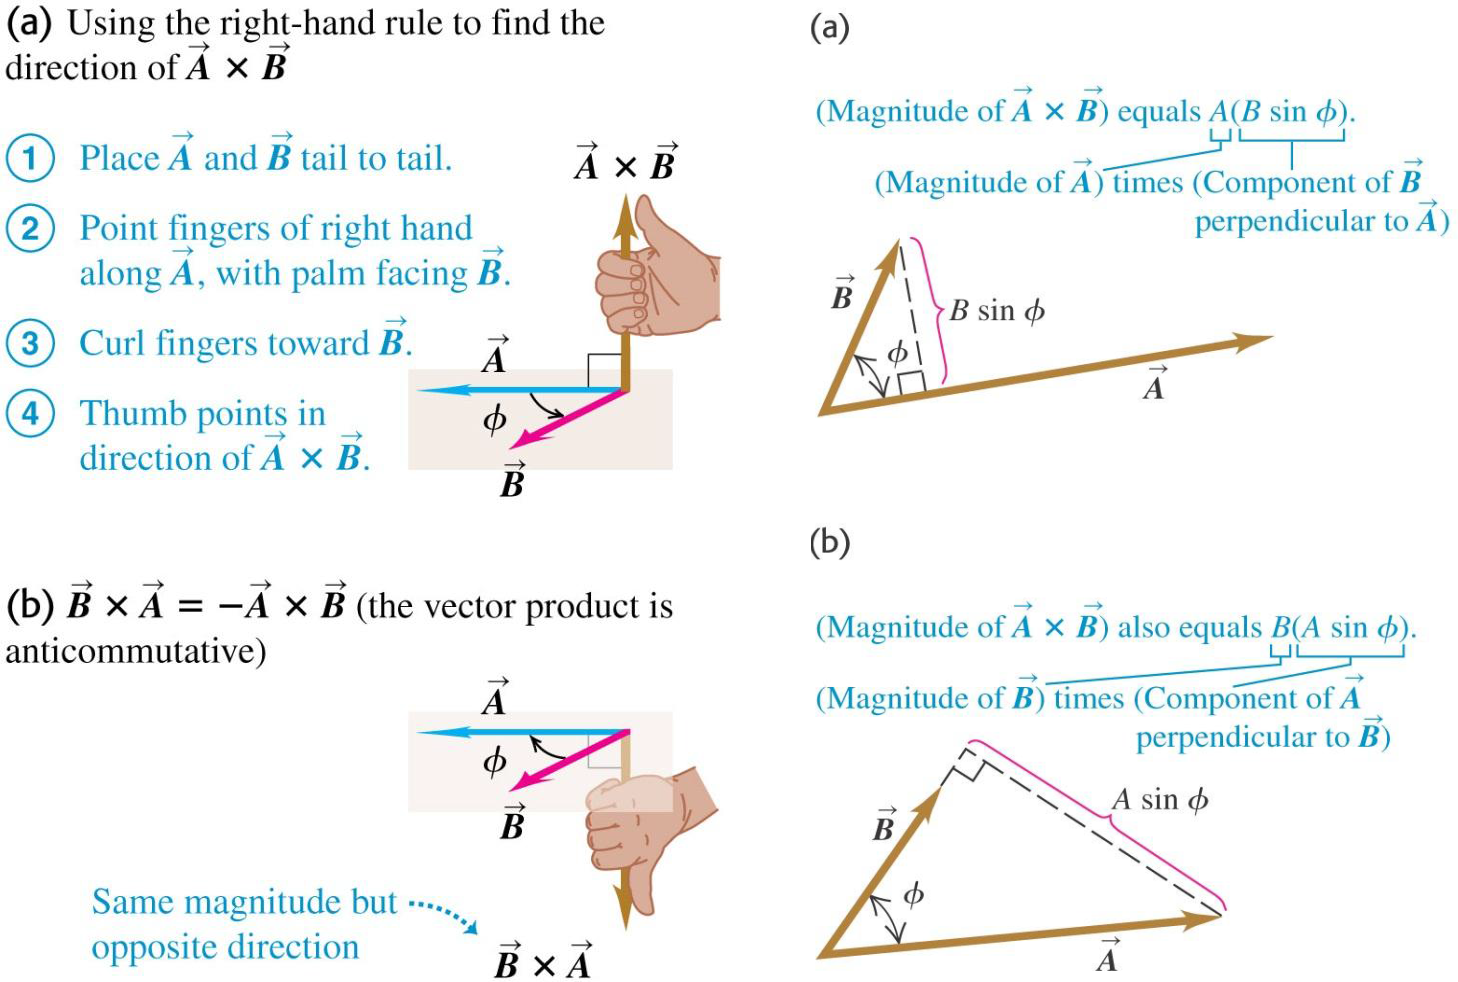
\includegraphics[width=\linewidth]{Vector_prod}
		\end{center}
	\end{column}
\end{columns}

\end{frame}
%=======================================================================================================

\end{document}

